\documentclass[a4paper, 12pt,twoside]{book}

% set the paper size and the margins
\usepackage[top = 2cm, bottom = 2cm, left = 2cm, right = 4cm ]{geometry}
\usepackage[showboxes]{textpos}
\setlength{\TPHorizModule}{10mm}
\setlength{\TPVertModule}{\TPHorizModule}
\TPMargin{2mm}
% set the header and the footnote
\usepackage{fancyhdr}
% Supress the hyphenation
\hyphenation{thatshouldnot}
% for table and equations
\usepackage{tablefootnote}
\usepackage{amsmath,amsfonts,amsthm}
\usepackage{multirow}
\usepackage{hhline}
% make a wide hat for the least-squares regression line
 \usepackage{scalerel,stackengine}
\stackMath
\newcommand\reallywidehat[1]{%
\savestack{\tmpbox}{\stretchto{%
  \scaleto{%
    \scalerel*[\widthof{\ensuremath{#1}}]{\kern-.6pt\bigwedge\kern-.6pt}%
    {\rule[-\textheight/2]{1ex}{\textheight}}%WIDTH-LIMITED BIG WEDGE
  }{\textheight}% 
}{0.5ex}}%
\stackon[1pt]{#1}{\tmpbox}%
}
\usepackage[shortlabels]{enumitem}

% knitr packages
\usepackage[]{graphicx}
\usepackage[]{color}
%% maxwidth is the original width if it is less than linewidth
%% otherwise use linewidth (to make sure the graphics do not exceed the margin)
\makeatletter
\def\maxwidth{ %
  \ifdim\Gin@nat@width>\linewidth
    \linewidth
  \else
    \Gin@nat@width
  \fi
}
\makeatother

\definecolor{fgcolor}{rgb}{0.345, 0.345, 0.345}
\newcommand{\hlnum}[1]{\textcolor[rgb]{0.686,0.059,0.569}{#1}}%
\newcommand{\hlstr}[1]{\textcolor[rgb]{0.192,0.494,0.8}{#1}}%
\newcommand{\hlcom}[1]{\textcolor[rgb]{0.678,0.584,0.686}{\textit{#1}}}%
\newcommand{\hlopt}[1]{\textcolor[rgb]{0,0,0}{#1}}%
\newcommand{\hlstd}[1]{\textcolor[rgb]{0.345,0.345,0.345}{#1}}%
\newcommand{\hlkwa}[1]{\textcolor[rgb]{0.161,0.373,0.58}{\textbf{#1}}}%
\newcommand{\hlkwb}[1]{\textcolor[rgb]{0.69,0.353,0.396}{#1}}%
\newcommand{\hlkwc}[1]{\textcolor[rgb]{0.333,0.667,0.333}{#1}}%
\newcommand{\hlkwd}[1]{\textcolor[rgb]{0.737,0.353,0.396}{\textbf{#1}}}%
\let\hlipl\hlkwb
\usepackage{framed}
\makeatletter
\newenvironment{kframe}{%
 \def\at@end@of@kframe{}%
 \ifinner\ifhmode%
  \def\at@end@of@kframe{\end{minipage}}%
  \begin{minipage}{\columnwidth}%
 \fi\fi%
 \def\FrameCommand##1{\hskip\@totalleftmargin \hskip-\fboxsep
 \colorbox{shadecolor}{##1}\hskip-\fboxsep
     % There is no \\@totalrightmargin, so:
     \hskip-\linewidth \hskip-\@totalleftmargin \hskip\columnwidth}%
 \MakeFramed {\advance\hsize-\width
   \@totalleftmargin\z@ \linewidth\hsize
   \@setminipage}}%
 {\par\unskip\endMakeFramed%
 \at@end@of@kframe}
\makeatother


\definecolor{shadecolor}{rgb}{.97, .97, .97}
\definecolor{messagecolor}{rgb}{0, 0, 0}
\definecolor{warningcolor}{rgb}{1, 0, 1}
\definecolor{errorcolor}{rgb}{1, 0, 0}
\newenvironment{knitrout}{}{} % an empty environment to be redefined in TeX

\usepackage{alltt}


% packages will be used by the 'kable' package
\usepackage{booktabs}
\usepackage{longtable}
\usepackage{array}
\usepackage{multirow}
\usepackage[table]{xcolor}
\usepackage{wrapfig}
\usepackage{float}
\usepackage{colortbl} 
\usepackage{pdflscape}
\usepackage{tabu}
\usepackage{threeparttable}
\usepackage{threeparttablex}
\usepackage[normalem]{ulem}
\usepackage{makecell}
\usepackage{xcolor}
\IfFileExists{upquote.sty}{\usepackage{upquote}}{}

% define a color for highlight
\definecolor{asparagus}{rgb}{0.53, 0.66, 0.42}
\definecolor{babypink}{rgb}{0.96, 0.76, 0.76}
\definecolor{champagne}{rgb}{0.97, 0.91, 0.81}
\definecolor{forestgreen}{rgb}{0.13, 0.55, 0.13}
\definecolor{dollarbill}{rgb}{0.52, 0.73, 0.4}

\usepackage{tcolorbox}

\tcbset{width=0.9\textwidth,boxrule=0pt,colback=champagne,arc=0pt,
auto outer arc,left=0pt,right=0p}

\usepackage{hhline}

\usepackage{amsmath}


\begin{document}

%Deal with the headers of each chapter
\pagestyle{fancy}
\fancyhf{}
\renewcommand{\chaptermark}[1]{ \markboth{#1}{} }
\fancyhead[CE,CO]{\leftmark}
\fancyfoot[LE,RO]{\thepage}

\chapter{Probabilities}

A lot of the times in our daily life, we can not predict the outcome of an event exactly, because of the complicated situations and the knowledge we don't know. However if this event is repeated many times, we may be able to calculate the "likelihood" of certain outcome, and this "likelihood" is called \textit{probability}.
\newpage

\section{\large{Probability and simulation}}
\vspace{0.3cm}

\textbf{Definition of probability}
\vspace{0.3cm}\\
When throw a coin, we say the probability of getting a \textit{head} is $0.5$. What does this mean? One way to interpret this is that: if we throw a fair coin many many time, half of the time will come up with a head. This is the \textbf{frequentists'} view of probability. The other way to interpret is: If a coin is tossed, the strength of your belief that it will come up with a \textit{head} is 0.5 if the strength of your belief is measured by numbers between 0 and 1. This is the \textbf{Baysian} view of probability.
\vspace{0.6cm}\\
\colorbox{babypink}{\parbox{\textwidth}{
 In this book and the AP exam we hold to the frequentists' view of probability.
}}
\vspace{0.3cm}\\
The \textbf{probability} of an outcome of a trial is defined as the relative frequency of this outcome if the trial is repeated many many times. 
\vspace{0.3cm}\\
If we want know the probability of getting a head when tossing a fair coin, we toss the coin millions of billions of times and calculate the ratio of the number of heads to the total number of trials.
\vspace{0.3cm}\\
Now the problem is how do we know that the \textit{relative} frequency converges as the number of trials increases. The \textbf{law of large numbers} guarantees the convergence, which says the limit of the relative frequency exists as the number of trials increases.
\vspace{0.6cm}\\
\textbf{Simulation}
\vspace{0.3cm}\\
The definition of the probability gives us a way to calculate the probability simply by repeating the trials. If you want find out the probability of getting a head, just tossing a coin many many times and calculate the relative frequency. However this is time consuming and sometimes not practical. We can simulate the process of tossing coins.
\vspace{0.3cm}\\
We can use a random number generator or table of random digits to generate random numbers between 0 and 9, if the number generated is between from 0 to 4, we take it as head, otherwise as tail. We generate the random numbers many many times and calculate the relative frequency of numbers from 0 to 4. This is more like an \textbf{experimentation} of probability. We call this process \textbf{simulation}.
\vspace{0.3cm}\\
\newpage


\colorbox{champagne}{\parbox{\textwidth}{
\textbf{Golden Ticket Parking Lottery}
\vspace{0.3cm}\\
At a local high school, 95 students have permission to park on campus. Each month, the student council holds a “golden ticket parking lottery” at a school assembly. The two lucky winners are given reserved parking spots next to the school’s main  entrance. Last month, the winning tickets were drawn by a student council member from the AP\textsuperscript{\textregistered} Statistics class. When both golden tickets went to members of that same class, some people thought the lottery had been rigged. There are 28 students in the AP Statistics class, all of whom are eligible to park on campus. Design and carry out a simulation to decide whether it’s plausible that the lottery was carried out fairly.
}}
\newpage

\section{\large{Probability models}}
\vspace{0.3cm}
\textbf{A little bit of counting}
\vspace{0.3cm}\\

    \begin{enumerate}
        \item \textbf{Principle of multiplication}
        \vspace{0.3cm}\\
       Ways from \textbf{A} to \textbf{C} is shown in figure \ref{PrincipleOfMultiplicatioin}, there are three ways from \textbf{A} to \textbf{B}, and there there are two ways from \textbf{B} to \textbf{C}. And, no matter which way is chosen from \textbf{A} to \textbf{B}, there are always 2 ways to choose from \textbf{B} to \textbf{C}. 
       \begin{figure}[H]
           \centering
           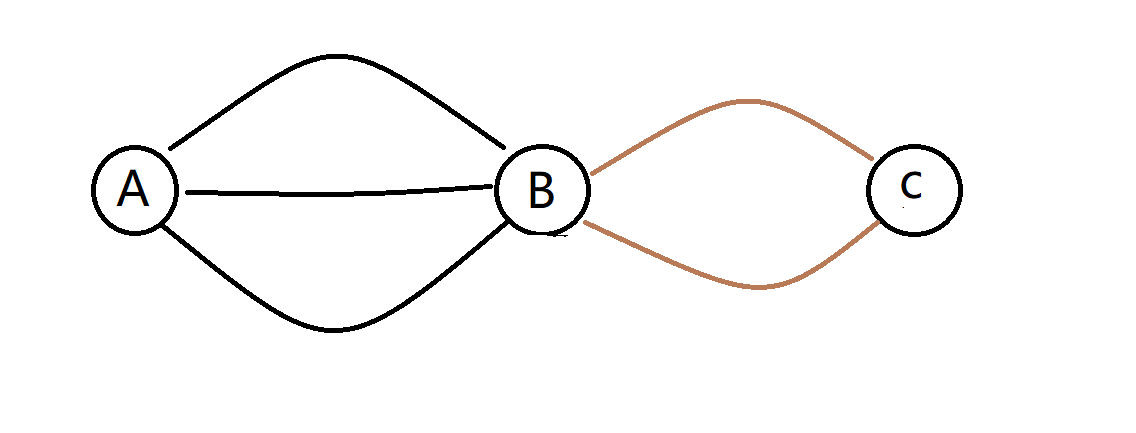
\includegraphics[scale=0.6]{PrincipleOfMultiplicatioin}
           \caption{Principle of multiplication}
           \label{PrincipleOfMultiplicatioin}     
       \end{figure}
       
   To find the total number of possible ways from \textbf{A} to \textbf{C}, just do multiplication.
   $$\textbf{Total number of ways} = 3 \times 2 = 6$$
   The above is called \textbf{\textit{principle of multiplication}}.
   
   \begin{textblock}{4}(-3.5, -2)
\textblockcolor{dollarbill}
\noindent
How many subsets are there for a set with $n$ elements?\\
\end{textblock}
\vspace{0.8cm}
   
   \item \textbf{Permutation}
   \vspace{0.3cm}
   
   \textbf{\textit{Permutation}} is to arrange a number of distinct elements in \textit{order}. For example, we want selected 3 out of 6 and arrange them in order. How many possible arrangements are there?
   \begin{figure}[H]
       \centering
       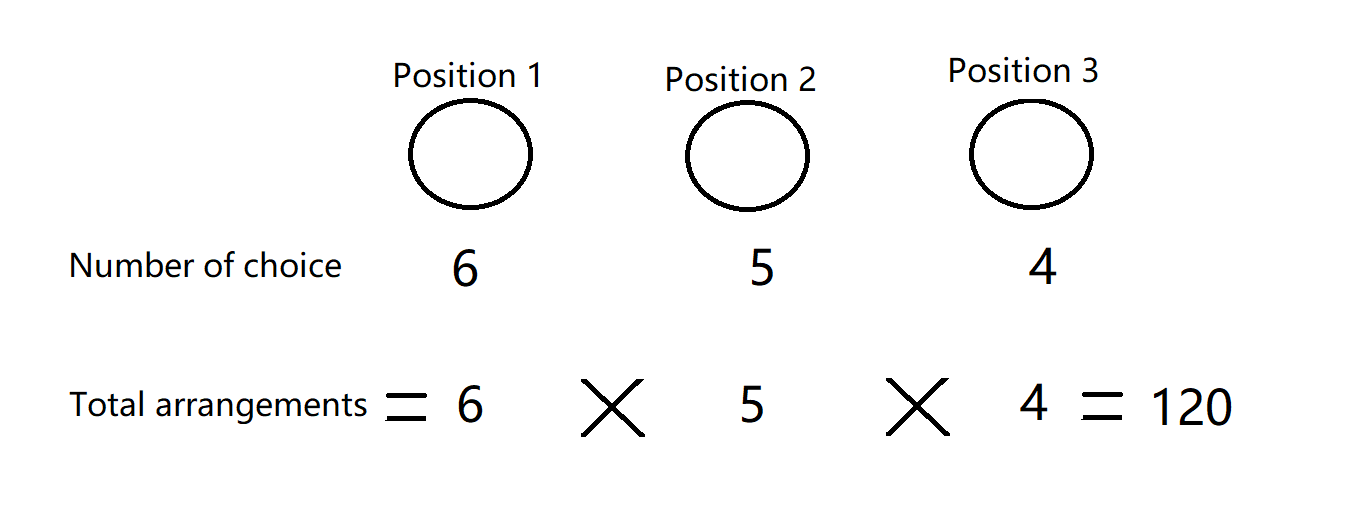
\includegraphics[scale=0.5]{Permutation}
       \caption{Permutation}
       \label{Permutation}
   \end{figure}
     As shown in figure \ref{Permutation}, first we fix three positions, then we fill out those positions one by one. There are 6 choices for position 1, 5 for position 2 and 4 for position 3. And no matter what choice is made in position 1, the number of choices for position 2 is the same. The same situation is true for position 2 and position 3. Thus, by applying the \textit{multiplication principle} the total number of arrangements is given by 
     $$6\times 5 \times 4 = 120.$$
     
     The above number of arrangement can be represented by notation $_3\textbf{P}_6$, where \textbf{P} means \textit{permutation}. 
     $$_m\textbf{P}_n = n \times (n-1) \times \dots \times (n-m+1)$$
     
     The total arrangements of arranging $n$ distinct elements in order can be represented by notation $n!$, read as \textbf{n factorial}.
     $$n! = n\times (n-1) \times \dots \times 2 \times 1$$
     \vspace{0.2cm}
     
        \item \textbf{Combination}
        
    Select $m$ elements out of $n$ distinct elements, without arranging them in order, is called \textbf{combination}. The notation is $_m\textbf{C}_n$.
    \vspace{0.3cm}
    
    Select 3 out of 6 elements and arrange the selected 3 in order. This is a permutation problem and the solution is given by $_3\textbf{P}_6$. Now lets solve this problem in another way. We divide the process into two steps. First, select 3 out of 6, which is a \textit{combination} problem, and the total combinations is denoted as $_3\textbf{C}_6$. Second, arrange the selected 3 in order. No matter how the 3 elements in selected in the first step, there will always be $3!$ arrangements for the second step. Apply the \textit{multiplication principle}.
    $$_3\textbf{P}_6 = _3\textbf{C}_6 \times 3!$$.
 Thus,
 \begin{equation*}
 \begin{split}
 _3\textbf{C}_6 &= \frac{_3\textbf{P}_6 }{3!} = \frac{6\times 5 \times 4}{3!} = \frac{6!}{3!\,3!}
 \end{split}
 \end{equation*}
 Similarly $$_m\textbf{C}_n = \frac{n!}{m!\,(n-m)!}.$$
    \vspace{0.3cm} 
    
    \colorbox{champagne}{\parbox{\textwidth}{
    \textbf{Prove:}  $_m\textbf{C}_n = _{n-m}\textbf{C}_n$
    }}  
    \end{enumerate}
    \newpage

\noindent   
\textbf{Probability models}    
\vspace{0.3cm}

Toss a coin, if it comes up with a head, we denote it as "H". If it if tail, it is denoted as "T". We toss a coin twice, and order matters. All possible outcomes can be given by the following set.
$$\textbf{S} = \{\text{(H,H), (H,T), (T,H),(T,T)}\}$$
The set of all possible outcomes is called the \textbf{sample space}, often denoted as \textbf{S}.
A \textbf{probability model} consists of the sample space and the probabilities assigned to each outcome.
\vspace{0.6cm}\\
An \textbf{event} is a subset of the sample space. For example event \textbf{A} can be given by 
         $$\textbf{A} = \{(H,H),(H,T), (T,H)\} $$
 Clearly $\textbf{A} \subset \textbf{S}$, and event \textbf{A} can be interpreted as "tossing a coin twice, and get at least one head". Operations of sets can be applied to events. $\textbf{P}(\textbf{A}\cup \textbf{B})$  means the probability that either \textbf{A}  or \textbf{B} happens. $\textbf{P}(\textbf{A}\cap \textbf{B})$  means the probability that both \textbf{A}  and \textbf{B} happen. 
    \vspace{0.6cm}\\    
 If all possible outcomes are equally likely, then we say this probability model is a \textbf{classical probability model}.
 \vspace{0.6cm}\\ 
When tossing a coin twice, and $\textbf{S} = \{\text{(H,H), (H,T), (T,H),(T,T)}\}$, each outcome has a probability 0.25. It is a \textit{classical probability model}.
\vspace{0.6cm}\\
If we toss a coin twice, and the sample space is given by $\textbf{S} = \{\text{(H,H), (H,T),(T,T)}\}$. In this case we assign probability 0.5 to outcome $(H,T)$, which means we don't distinguish the order of the tossing, $(H,T)$ and $(T,H)$ are the same outcome. In this case, it is not a \textit{classical probability model}.
\vspace{0.6cm}\\
For classical probability model, the probability of an event \textbf{A} can be given by 
    $$\textbf{P}(\textbf{A}) = \frac{n(\textbf{A})}{n(\textbf{S})},$$
    where $n(\textbf{A})$ means the number of outcomes in \textbf{A}, and $n(\textbf{S})$  means the total number of outcomes.
    \vspace{0.6cm}\\
    
\begin{textblock}{3.3}(-3.6, -6)
\textblockcolor{dollarbill}
\noindent
There will either be an earthquake or not, only two outcomes. Thus the probability of having an earthquake tomorrow is 1/2. What is wrong with this argue?\\
\end{textblock}
\hspace{-0.5cm}
\colorbox{champagne}{\parbox{\textwidth}{
    \textbf{Exercise:}\\
    Toss a die twice. Find the following probabilities.
    \begin{enumerate}[(a)]
        \item Event \textbf{A}:the sum is divisible by 2.
        \item Event \textbf{B}:the sum is divisible by 3.
        \item Event \textbf{C}:the sum is divisible by 5.
        \item $\textbf{A} \cup \textbf{B}$. Interpret the meaning of this event.
        \item $\textbf{A} \cap \textbf{B}$. Interpret the meaning of this event.
        \item $\textbf{A} \cap \textbf{C}$.Interpret the meaning of this event.
    \end{enumerate}   
}}
\newpage

\section{\large{Probability rules}}
\textbf{General addition rule}
\vspace{0.3cm}

    Since events are subsets of sample space \textbf{S}, there relations can be represented by the \textit{Venn Diagram} as shown in figure \ref{GeneralAdditionRule}. Lets simply take the probabilities of different events as areas enclosed by different events, and $\textbf{P}(\textbf{S}) = 1$.
    \begin{figure}[H]
    \centering
    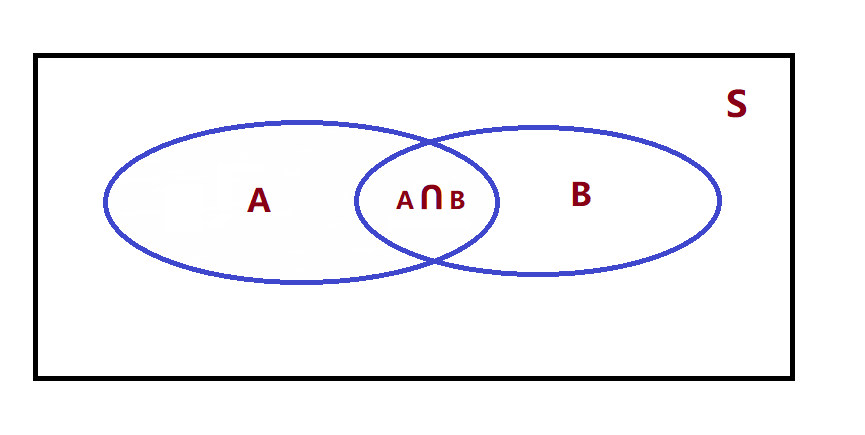
\includegraphics[scale=0.6]{GeneralAdditionRule}
    \caption{General addition rule}
    \label{GeneralAdditionRule}    
    \end{figure}
    
According to the \textit{Venn Diagram}, we have 
    $$\textbf{P}(\textbf{A} \cup \textbf{B}) = \textbf{P}(\textbf{A}) + \textbf{P}(\textbf{B}) - \textbf{P}(\textbf{A} \cap \textbf{B}).$$
    
\noindent  The above is called the \textbf{general addition rule}. If $ \textbf{P}(\textbf{A} \cap \textbf{B}) = 0$, we say \textbf{A} and \textbf{B} are \textbf{mutually exclusive}, which means they can not happen at the same time.
  \vspace{0.3cm}\\
  If \textbf{A} and \textbf{B} are \textit{mutually exclusive}, then 
    $$\textbf{P}(\textbf{A} \cup \textbf{B}) = \textbf{P}(\textbf{A}) + \textbf{P}(\textbf{B}) .$$
  
  
 \noindent  $\textbf{A}^C$ is the \textbf{complementary} of \textbf{A},  
  $\textbf{P}(\textbf{A} \cap \textbf{A}^C) = \textbf{P}(\emptyset) = 0$. Thus
   
  $$\textbf{P}(\textbf{S})= \textbf{P}(\textbf{A}) + \textbf{P}(\textbf{A}^C) - \textbf{P}(\textbf{A} \cap \textbf{A}^C) = 1.$$
\vspace{0.6cm}\\
\colorbox{champagne}{\parbox{\textwidth}{
    \textbf{Exercise:}\\
    Toss a die twice.\\
    Event \textbf{A} means "the sum is divisible by 2".\\
    Event \textbf{B} means "the sum is divisible by 3".\\
    Event \textbf{C} means "the sum is divisible by 5".\\
    \begin{enumerate}[(a)]
        \item Which of the following pairs of events are mutually exclusive?\\
        (1) \textbf{A}, \textbf{B} \hspace{0.6cm} (2) \textbf{A}, \textbf{C} \hspace{0.6cm} (3) \textbf{B}, \textbf{C}.        
        \item Find $\textbf{P}(\textbf{A} \cup \textbf{B})$, 
           $ \textbf{P}(\textbf{A} \cup \textbf{C})$,
           $ \textbf{P}(\textbf{B} \cup \textbf{C})$.        
    \end{enumerate}   
}}
\newpage

\noindent
\textbf{General multiplication rule}
\vspace{0.3cm}\\
Take a look at this example. Randomly select 178 students, and check whether they have got their ear pierced. The results is give by figure \ref{EarPierced}.
    \begin{figure}[H]
        \centering
        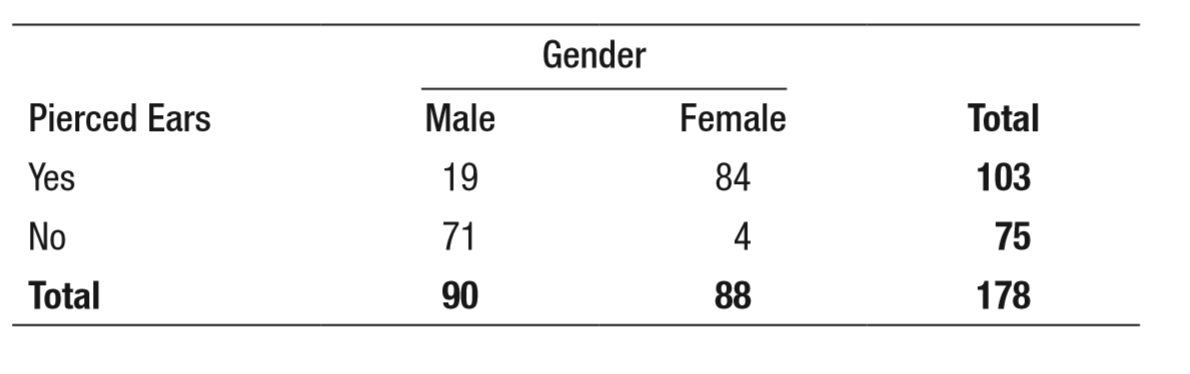
\includegraphics[scale=0.6]{EarPierced}
        \caption{Data of pierced ears}
        \label{EarPierced}
    \end{figure}
Let's denote event \textbf{A} as "male" and event \textbf{B} as "pierced ears". For a randomly chosen students, the probability that his/her ears are piecered is $$\textbf{P}(\textbf{B}) = \frac{103}{178}.$$
If we tweak the situation a little bit and ask "For a randomly chosen student, we know he is male, what is the probability his ears are pierced?" Since we already know this student is male, we only have to consider the probability among the group of male students. In this male group, the probability that his ears are pierced is $\displaystyle{\frac{19}{90}}$. We call this kind of probability \textbf{conditional probability}, and denoted as $\textbf{P}(\textbf{B}|\textbf{A})$, which means the probability of \textbf{B}("pierced ears") on condition that \textbf{B} happened("male"). We have the following formulae:
$$\textbf{P}(\textbf{A} \cap \textbf{B}) = \textbf{P}(\textbf{A}) \cdot \textbf{P}(\textbf{B}|\textbf{A})= \textbf{P}(\textbf{B}) \cdot \textbf{P}(\textbf{A}|\textbf{B}).$$
$$\textbf{P}(\textbf{B}|\textbf{A}) = \frac{\textbf{P}(\textbf{A} \cap \textbf{B})}{\textbf{P}(\textbf{A})}.$$

\begin{textblock}{4}(-3, -2)
\textcolor{dollarbill}
Calculate $\textbf{P}(\textbf{A}|\textbf{B})$ and interpret its meaning.
\end{textblock}

\hspace{-0.5cm}
\colorbox{babypink}{\parbox{\textwidth}{
  Those formulae are very important. They play a key role in \textbf{Baysian statistics} as well.
}}
\vspace{0.6cm}

If $\textbf{P}(\textbf{B} | \textbf{A})=\textbf{P}(\textbf{B})$, we say \textbf{A} and \textbf{B} are \textbf{independent}, which means whether \textbf{A} happens or not, it won't influence the probability of \textbf{B}. In fact 
$$\textbf{P}(\textbf{B} | \textbf{A})=\textbf{P}(\textbf{B})
   \implies \textbf{P}(\textbf{A} | \textbf{B})=\textbf{P}(\textbf{A})$$
   This means \textit{independence} is \textit{mutual}. If \textbf{A} is independent of \textbf{B}, then \textbf{B} is independent of \textbf{A}.
   \vspace{0.6cm}

\hspace{-0.5cm}
 \colorbox{champagne}{\parbox{\textwidth}{
 \textbf{Prove:}\hspace{0.6cm}$\textbf{P}(\textbf{B} | \textbf{A})=\textbf{P}(\textbf{B})
   \implies \textbf{P}(\textbf{A} | \textbf{B})=\textbf{P}(\textbf{A})$
 }}
\newpage
If \textbf{A} and \textbf{B} are independent, then $$\textbf{P}(\textbf{A} \cap \textbf{B}) = \textbf{P}(\textbf{A}) \cdot \textbf{P}(\textbf{B})$$. 
\noindent This formula can be generalized to more than two independent events.
\vspace{0.6cm}\\

\hspace{-0.5cm}
\colorbox{champagne}{\parbox{\textwidth}{
 \textbf{The Challenger Disaster?}
 \vspace{0.3cm}\\
 On January 28, 1986, Space Shuttle Challenger exploded on takeoff. All seven crew members were killed. Following the disaster, scientists and statisticians helped analyze what went wrong. They determined that the failure of O\textendash ring joints in the shuttle’s booster rockets was to blame. Under the cold conditions that day, experts estimated that the probability that an individual O\textendash ring joint would function properly was 0.977. But there were six of these O-ring joints, and all six had to function properly for the shuttle to launch safely.
 \vspace{0.3cm}\\
  Assuming that O\textendash ring joints succeed or fail independently, find the probability that the shuttle would not launch safely under similar conditions.
  }}
\newpage



\noindent \textbf{Tree diagram and conditional probability}
\vspace{0.6cm}\\
\hspace{-0.5cm}
\colorbox{champagne}{\parbox{\textwidth}{
 \textbf{Who Visits \textit{YouTube}?}
 \vspace{0.3cm}\\
 Video\textendash sharing sites, led by YouTube, are popular destinations on the Internet. Let’s look only at adult Internet users, aged 18 and over. About 27\% of adult Internet users are 18 to 29 years old, another 45\% are 30 to 49 years old, and the remaining 28\% are 50 and over. The Pew Internet and American Life Project finds that 70\% of Internet users aged 18 to 29 have visited a video\textendash sharing site, along with 51\% of those aged 30 to 49 and 26\% of those 50 or older. 
 \vspace{0.3cm}\\
 Suppose we select an adult Internet user at random. 
 \begin{enumerate}
     \item Find the probability that this person has visited a video\textendash sharing site.Show your work.
     \item Given that this person has visited a video\textendash sharing site, find the probability that he or she is aged 18 to 29. Show your work.
 \end{enumerate}
 }}
 \newpage
 




\end{document}